\chapter{Catching Attackers in Restricted Network Zones}
\label{chap:concept}

The T-Pot identified a flood of threats when it was available on the Internet.
However, capacious networks have separated compartments, and services are usually not directly available without any protection.
Zoning is a well-known method to segment a network.
Heidelberg University applies zoning, and thus, it is an interesting question if an attacker probes services outside or within the network.
This chapter presents a concept that uses a honeypot-like detection tool to detect any dubious packets in the network.
It shows that attacks in a restricted network zone of the Heidelberg University's internal network occurred and contributed to an adaption of the stateless firewall.
Thus, improving the security of the network.

\section{University Network}

Honeypots that are accessible via the Internet receive a broad range of attacks.
As \citet{Spitzner2003} noted, a honeypot is not strictly bound to run in a \ac{dmz} or a network with direct Internet access.
The correct location has to be chosen based on the goals of the honeypot.
For example, one goal could be to catch attackers behind a perimeter firewall to reveal leaks or vulnerabilities.
Beforehand, the honeypot was broadly available on the Internet, and attackers could probe it easily.
It collected on average \numprint{29840} attacks per day, resulting in a total amount of \numprint{607747} attacks.
Zoning a network into logical groups mitigates the risk of an open network.
Thus, the T-Pot would receive significantly fewer attacks in a controlled network zone.
A network infrastructure is segmented into the same communication security policies and security requirements.
For example, the Canadian government created its baseline for infrastructures, called Baseline Security Architecture Requirements for Network Security Zones in the Government of Canada (ITSG-22).
The four most common zones are:
\begin{enumerate*}[label=(\roman*)]
    \item Public Zone (PZ), which is entirely open,
    \item Public Access Zone (PAZ), which interacts as an interface between the PZ and internal services,
    \item Operation Zone (OZ), which processes sensitive information, and
    \item Restricted Zone (RZ), which includes business-critical services
\end{enumerate*}.
A network zone restricts access and controls data communication flows. \cite{csec2021}

\begin{figure}
    \centering
    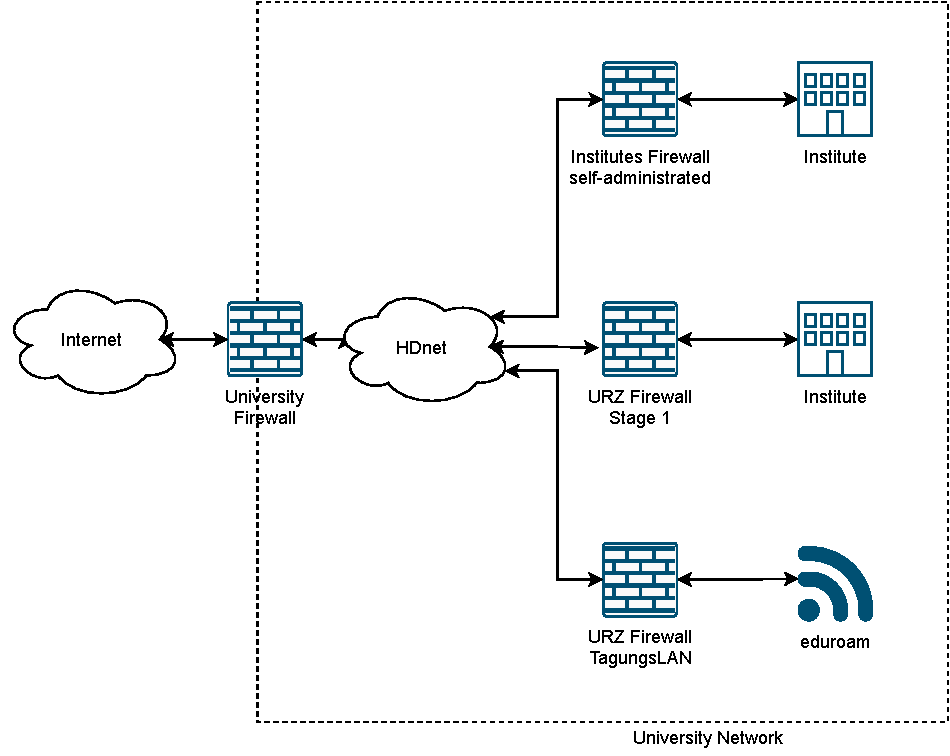
\includegraphics[width=\textwidth]{figures/university-network.pdf}
    \caption[Draft of the University network]{
        Draft of the University network.
        The main doorkeeper is the university firewall.
        The HDnet is the internal network allowing institutes to communicate with each other.
    }
    \label{fig:university-network}
\end{figure}

The network at the Heidelberg University includes a central stateless firewall (\ac{acl}) that enfolds all institutes.
It entails a default blacklist that blocks certain services (such as SMTP, NCP, or \ac{snmp}) and a stateless filter provided by BelWÜ.
Each institute can either use a pre-defined stateless firewall provided by the University Computing Center Heidelberg or use a self-administrated firewall inside the network.
\autoref{fig:university-network} outlines the association between these components.
The internal \enquote{HDnet} enables the communication between institutes without leaving the internal network.
Institute firewalls can be set up by each institute and are self-administrated.
They do have the possibility to use \acs{soho} routers\footnote{A \acl{soho} router is a broadband router used in small offices and home offices environments.} to disconnect certain network zones from the network.
It is recommended to configure the global \ac{acl} as a fallback solution in case of any downtime.
The University Computing Center Heidelberg offers stateless firewalls for router interfaces or VLANs.
This stateless firewall whitelists certain services and splits up into four stages.
Each stage can be individually activated per router interface.
Its key value is to maintain baseline security to avoid misconfigurations and port scans.
\autoref{tab:overview-security-zone} outlines these stages including the IP address range.
Before applying one of these zones, the respective network has to oblige to client IP addresses below \ipAddress{129.206.218.240/24}.
In addition, \ipAddress{129.206.218.1} is allocated for the gateway.
A network must adhere to these obligations if it applies to any pre-defined stages.

\begin{table}
    \centering
    \caption[Overview of firewall stages]{
        Overview of firewall stages at the Heidelberg University.
        As an example, it applies the rules to subnet \ipAddress{129.206.218.0/24}.
        Rules are applied to any subnet.
    }
    \begin{tabularx}{\linewidth}{l|XX}
        \toprule
        \textsc{Name} & \textsc{Description}                      & \textsc{range}                     \\
        \hline
        Stage 0       & Filters broadcast communication           & \ipAddress{129.206.218.0-15/24}    \\
                      & No filtering                              & \ipAddress{129.206.239.16-255/24}  \\
        \hline
        Stage 1       & Allows common network protocol            & \ipAddress{129.206.239.0-255/24}   \\
                      & Allows services                           & \ipAddress{129.206.239.240-255/24} \\
        \hline
        Stage 3       & Internet access only via internal proxies & \ipAddress{129.206.239.0-255/24}   \\
        \hline
        Stage 4       & Only internal network communication       & \ipAddress{129.206.239.0-255/24}   \\
        \bottomrule
    \end{tabularx}
    \label{tab:overview-security-zone}
\end{table}

An interesting question is if attackers have access to restricted zones at the Heidelberg University.
It arises during the research of T-Pot if an adversary would try to probe any hosts in the internal university network.
In order to detect such events, a honeypot-like packet detection application is presented that helps identify any threats in a network.
In addition, it offers to deploy multiple instances and collect their data at a centralized instance.

\section{Honeypot-like Connection Detection Tool}

Recording and investigating connection attempts assimilates new honeypots.
Respectively, a new honeypot-like detection tool called MADCAT will be presented.
MADCAT has been developed by the BSI and helps to log any connection attempt being made on the host machine.
The acronym MADCAT stands for \textit{Mass Attack Detection Connection Acceptance Tools}.
It works as a honeypot-like detection application with a low-interaction level.
Its key idea is to log every connection attempt and further process it to retrieve credentials or shell exploitation.
\autoref{fig:madcat-architecture} gives an insight how MADCAT works.
It runs on an Ubuntu distribution, either $18.04$ or $20.04$, and has been tested on Ubuntu $18.04$.
It processes packets from any interface that has been configured.
As an example, it could process Ethernet and wireless packets.
MADCAT itself consists of six independent modules for TCP, UDP, ICMP, and RAW packets that communicate with each other through a pipeline.
A module analyzes packets and logs the results in a queue.
In addition, UDP and TCP offer a proxy to tunnel packets to another service.
Every 5 seconds TCP postprocessor reads the newly arrived TCP packets and processes them accordingly.
It resolves packets to log data, including source IP address, protocol, and event type.
The enrichment processor is the final process step.
Its purpose is to log all queue-written packets in a specified format for further analysis.
The key idea of MADCAT is to get an insight into whether attackers have access to a particular network.
In contrast to T-Pot, the concept does not know what specific attacks are operated on the honeypot.
Instead, it ensures that no one else than authorized users has access.
Especially in high confidential areas, no attacker should be capable of sending even a single packet to a host in the network.
The vast range of honeypots does not provide tracking packets on a detailed level.

\begin{figure}
    \centering
    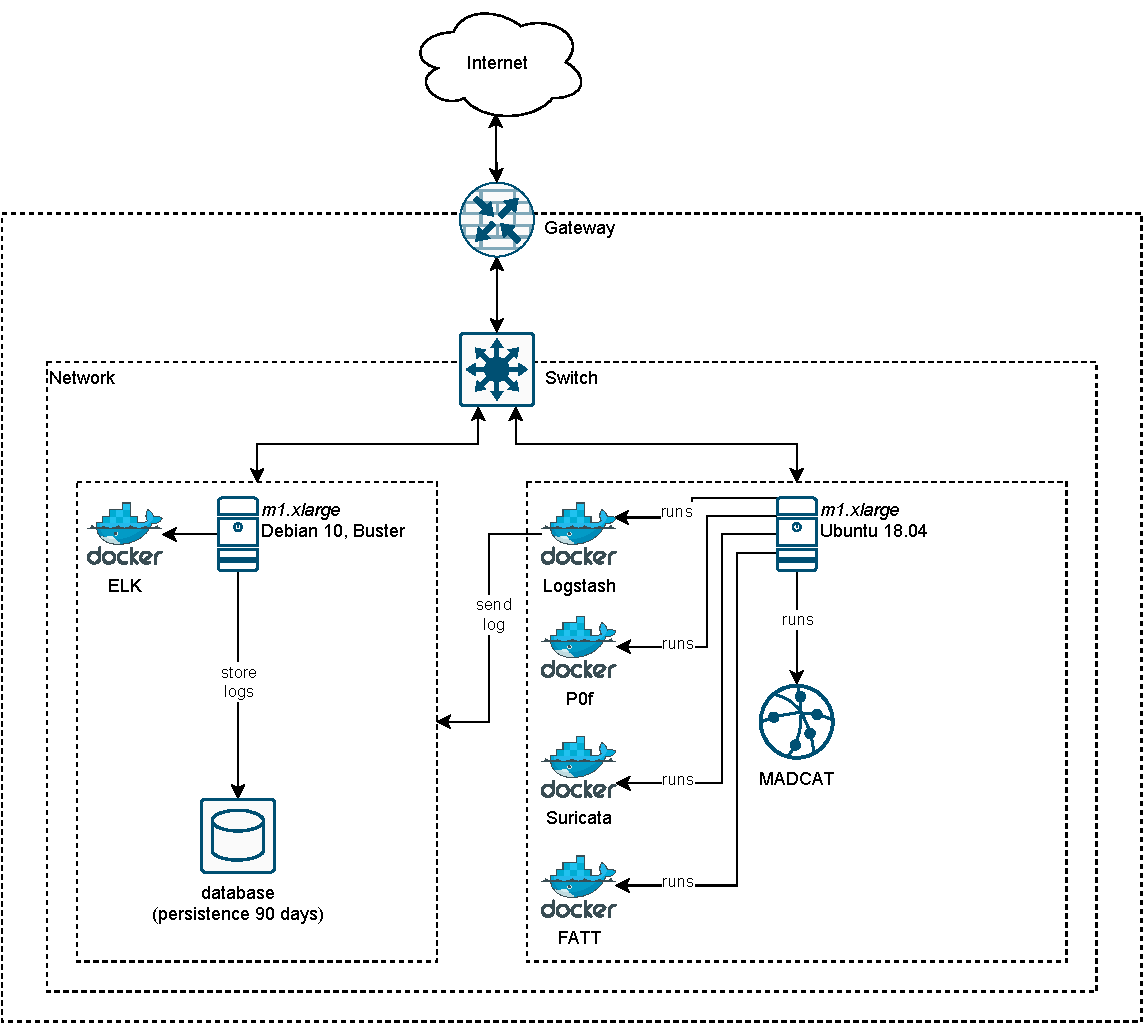
\includegraphics[width=\textwidth]{figures/heicat-concept.pdf}
    \caption[Concept to detect connection attempts]{
        Concept to detect connection attempts.
        It has been drafted to work in various scenarios.
        Kibana and Elasticsearch are deployed in heiCLOUD.
    }
    \label{fig:heicat-concept}
\end{figure}

In addition, a T-Pot instance will be deployed to have comparison data to the new concept.
It focuses on the \ipAddress{129.206.218.0/24} and \ipAddress{147.142.0.0/16} subnet.
The \ipAddress{129.206.218.0/24} subnet is used within University Computing Center Heidelberg building.
Every client in the building has a compelling connection in this subnet.
Otherwise, an Internet connection would not be feasible.
The subnet \ipAddress{147.142.0.0/16} connects clients to \enquote{eduroam}\footnote{The eduroam is an international Wi-Fi internet access point for researchers.}.
Like the four stages of the institute firewall, the \enquote{eduroam} network, also called \enquote{Tagungslan}, builds various permits into the subnet.
One essential difference is that services like SMTP and HTTP are not allowed, so attackers cannot deploy traps for users.
Moreover, each client is encapsulated in its subnet, which disables communication to other clients.
The instances are located in the building with IP addresses \ipAddress{129.206.219.62} and \ipAddress{129.206.219.88}.
\autoref{fig:heicat-concept} outlines the concept using MADCAT and a separate instance to visualize our data.
The first instance with IP address \ipAddress{129.206.5.157} provides Kibana and Elasticsearch to visualize and crawl logs.
The honeypot with IP address \ipAddress{129.206.5.88} consists of MADCAT in conjunction with P0f, Suricata, and FATT.
Like T-Pot, it uses Logstash to forward data to Elasticsearch.
One benefit is the centralized approach to store data.
This allows to deploy more instances to randomly collect data from other zones.

\begin{figure}
    \centering
    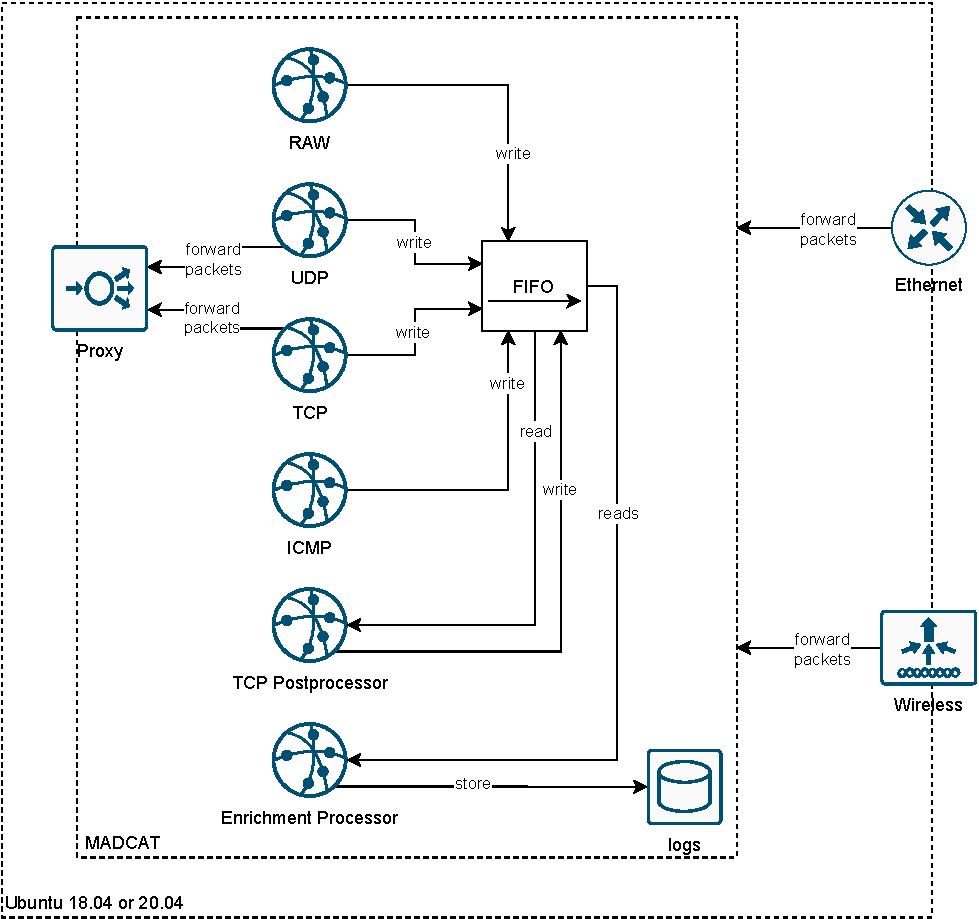
\includegraphics[width=\textwidth]{figures/heicat-architecture.pdf}
    \caption[Visualization of the MADCAT packet flow]{
        Visualization of the MADCAT packet flow starting at the network interface.
        The Ethernet and wireless interface forwards packets to the desired module.
    }
    \label{fig:madcat-architecture}
\end{figure}

\section{Results}

MADCAT (28th of October till 18th of November) and T-Pot (16th of November till 7th of December) have been deployed for three weeks.
All instances had a connection to both subnets.
First, the results obtained in the subnet \ipAddress{129.206.218.0/24} will be presented, closing up with the ones claimed in the eduroam network.

In total, MADCAT received \numprint{35372} packets.
Overall, the modules TCP ($66.62\%$) and RAW ($33.26\%$) received the majority of all connection attempts.
The minority with less than one percent are suspicious packets with individual TCP flags like reset or syn set. 
On the contrary, it could not identify any harmful activity based on these packets.
Overall, ConPot ($56.98\%$), Honeytrap ($31.35\%$), and Dionaea ($7.09\%$) received most of the attacks with a total number of $437$.
Interestingly, it could identify \ac{snmp} connections that are used by print servers to discover printers.

\begin{figure}
    \centering
    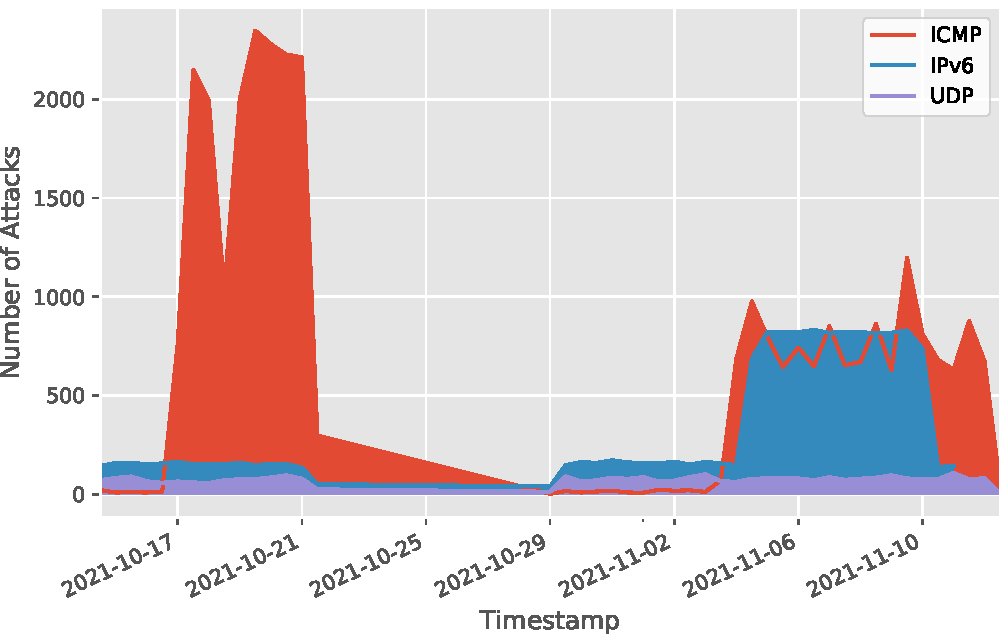
\includegraphics[width=\textwidth]{figures/madcat-protocol-usage.pdf}
    \caption[Protocol distribution of MADCAT]{
        Protocol distribution of MADCAT. ICMP, IPv6, and UDP are the most used protocols.
        Timestamp; 28th of October to 18th of November.
    }
    \label{fig:madcat-protocols}
\end{figure}

% ====================================================================================================================
% Madcat
\autoref{fig:madcat-protocols} shows the protocol distribution indicating a high amount of ICMP and IPv6 packets.
Only $11.59\%$ of all IP address reputations could be resolved, splitting up into known attacker ($11.26\%$), mass scanner ($0.14\%$), bad reputation ($0.12\%$), and tor exit node ($0.08\%$).
Focusing on TCP packets, $88.3\%$ are known attackers with source port 113 as the primary target.
The port 113 is officially known as the \ac{ident}\cite{rfc1413} used for identification/authorization on a remote server such as POP, IMAP, and SMTP.
A potential leak that allows adversaries to send IDENT requests to the network could be spotted by comparing the results with the stateless firewall settings.
Decoding the payload of these TCP packets shows that attackers instead used this port to get an SMB connection than deploying IDENT protocol attacks.
It identified attempts to acquire an SSH session using SMB and SIP connection attempts and various HTTP requests.
For example, two payloads that have been sent to the instance show probing actions.
\autoref{lst:sip-exploitation} outlines a SIP probe that checks if any VoIP service is active by answering the request packet.
Next, \autoref{lst:smb-exploitation} shows an SMB probe trying to achieve the same.
The IP address reputation could help answer if a real user or an attacker sends these packets.
Both IP addresses in this example were resolved as a known attacker; thus, it identified them as a probe packet before executing their attack.
A vital security interest in port 113 is negligible; however, the concept helps to detect such leaks, especially when stateless firewalls are the main doorkeeper for packets.

\begin{figure}
    \centering
    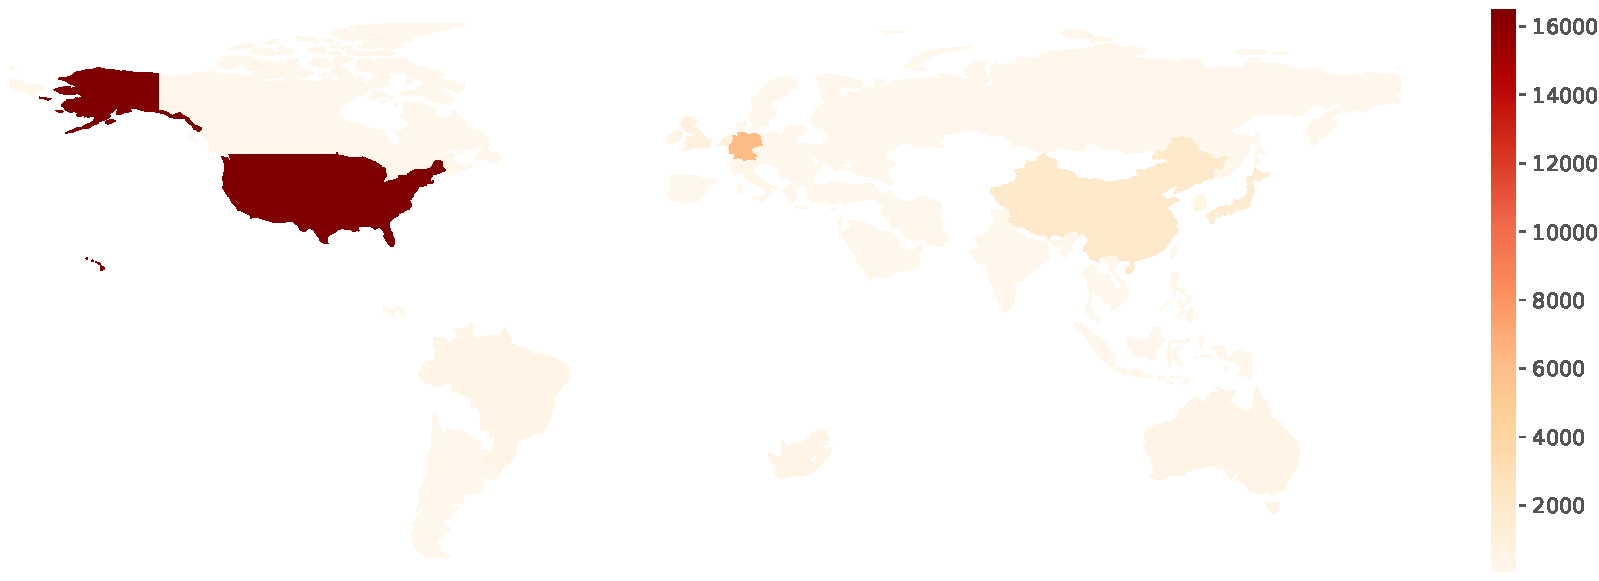
\includegraphics[width=\textwidth]{figures/madcat-overview-map.pdf}
    \caption[Attack distribution of MADCAT]{
        Attack distribution of MADCAT.
        USA, Russia, China, and Germany are the most attacking countries.
        Timestamp; 28th of October to 18th of November.
    }
    \label{fig:madcat-attack-distribution}
\end{figure}

% ====================================================================================================================
% Location
\autoref{fig:madcat-attack-distribution} shows the attack distribution indicating the origin of an IP address.
Most of the connections originate from the United States, Germany, and China.
As shown beforehand in \autoref{chap:cloud-security}, geographical information only outlines the last known location of a node.
Like the results in heiCLOUD, it can be assumed that this information is not reliable as an indicator of where attacks occur.
Nevertheless, it is interesting to see where the last node originated from.

\begin{figure}
    \centering
    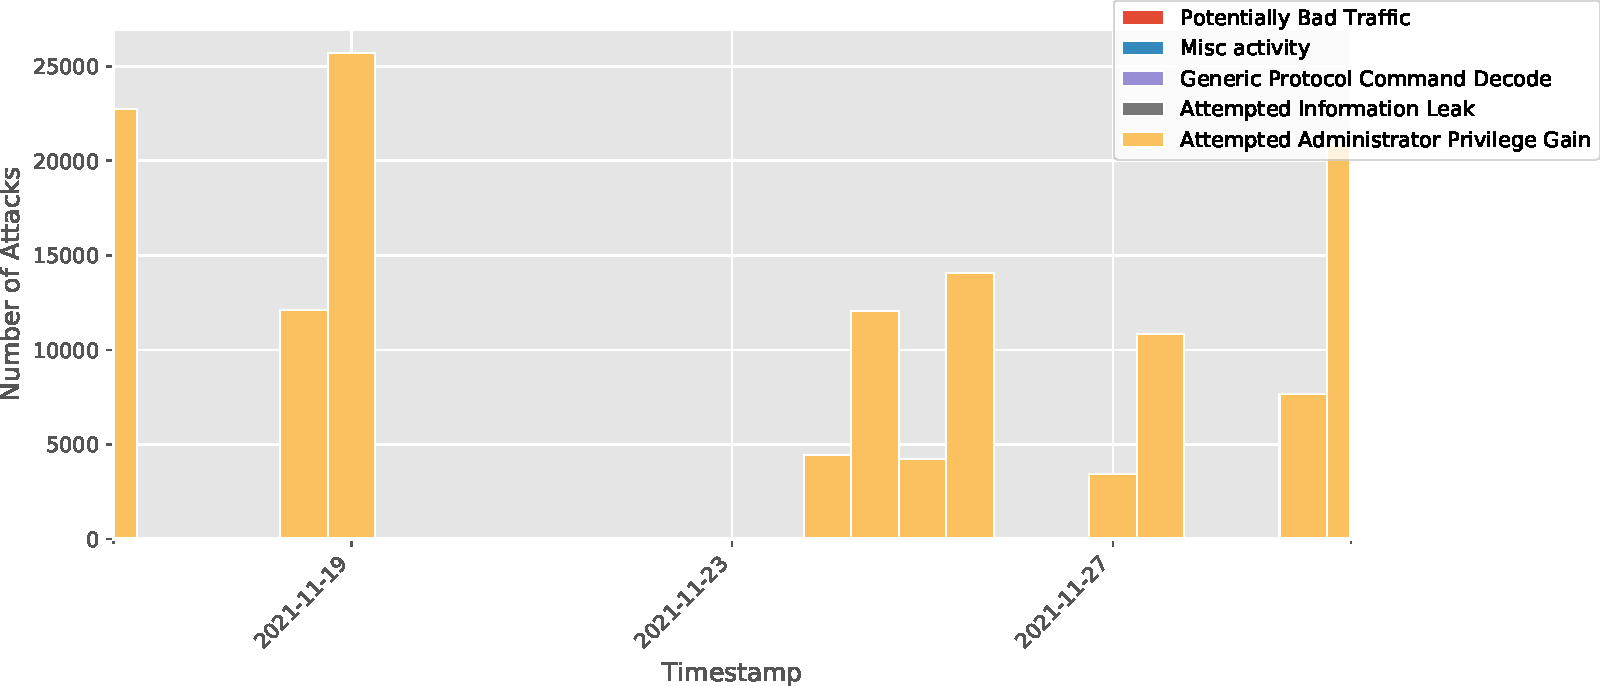
\includegraphics[width=\textwidth]{figures/madcat-suricata-alerts.pdf}
    \caption[Suricata results of T-Pot]{
        Suricata results of T-Pot.
        Timestamp; from 16th of November to 7th of December.
    }
    \label{fig:suricata-distribution}
\end{figure}

% ====================================================================================================================
% Suricata
Suricata identified odd behaviors in the network (\autoref{fig:suricata-distribution}).
In total, it detected \numprint{292953} alerts and \acsp{cve}.
Besides minor alerts like \textsc{nmap} scans, Suricata registered alerts in \ac{snmp} requests, TCP stack, and Wind River VxWorks.
CVE-2020-11899 \cite{CVE-2020-11899} accounts nearly $73.35\%$ with a total number of \numprint{214879}.
This \acs{cve} is one of 19 others forming the \enquote{Ripple20} vulnerability in the low-level TCP/IP library developed by Treck, Inc.
One of the Track TCP/IP stack tasks is to reassemble fragmented packets.
Whenever a fragmented packet arrives, the stack tries to validate the total length in the IP header.
If the total length is not correct, it trims the data.
However, this leads to inconsistency, and thus, resulting in a buffer overflow when someone sends fragmented packets through a tunnel.
A detailed description of the vulnerability can be found in \cite{ripple20}.
An adversary could send malformed IPv6 packets that cause an Out-of-bounds Read, resulting in potential remote code execution.
Only TCP/IP stack versions until $6.0.1.66$ are affected by this vulnerability.
Nevertheless, the tremendous alerts show the importance of adapting the IPv6 permits.
The second most recorded vulnerability with the highest score is CVE-2002-0013 \cite{CVE-2002-0013} that allows remote attackers to cause a denial of service or gain privileges in the SNMPv1 protocol.
The root cause for the \acs{cve} alert is the usage of the default public community for broadcast requests instead of configuring a private community with mandatory authentication.
To compromise \ac{snmp}, attackers have to have access to the network.
However, the university firewall blocks \ac{snmp} port 161 and 162 for TCP and UDP, thus, restricting any access from outside.
If adversaries plan to deploy an attack on the \ac{snmp} protocol, they need to have a connection to the internal network.
Acquiring such a connection is rather hard to accomplish without any credentials.
On the contrary, all connection attempts registered by the concept have been made within the network, and they do reflect a normal \ac{snmp} communication.
Lastly, Wind River VxWorks 6.9.4 and vx7 in CVE-2019-12263 \cite{CVE-2019-12263} cause a buffer overflow due to the underlying TCP component that results in a race condition.
Each connection attempt with CVE-2019-12263 is originated from Russia.
Hence, the assumption is that the source IP address maliciously intended to send an urgent flag.
For the other \acsp{cve} the IP reputation could not be resolved.

\begin{figure}
    \lstinputlisting[language=bash, caption={[MADCAT connection attempt to exploit SIP connection]MADCAT connection attempt to exploit SIP connection. Received on the 16th of November. IP reputation: known attacker. Location Germany.}, label={lst:sip-exploitation}]{listings/exploit-sip.txt}
\end{figure}

\begin{figure}
    \centering
    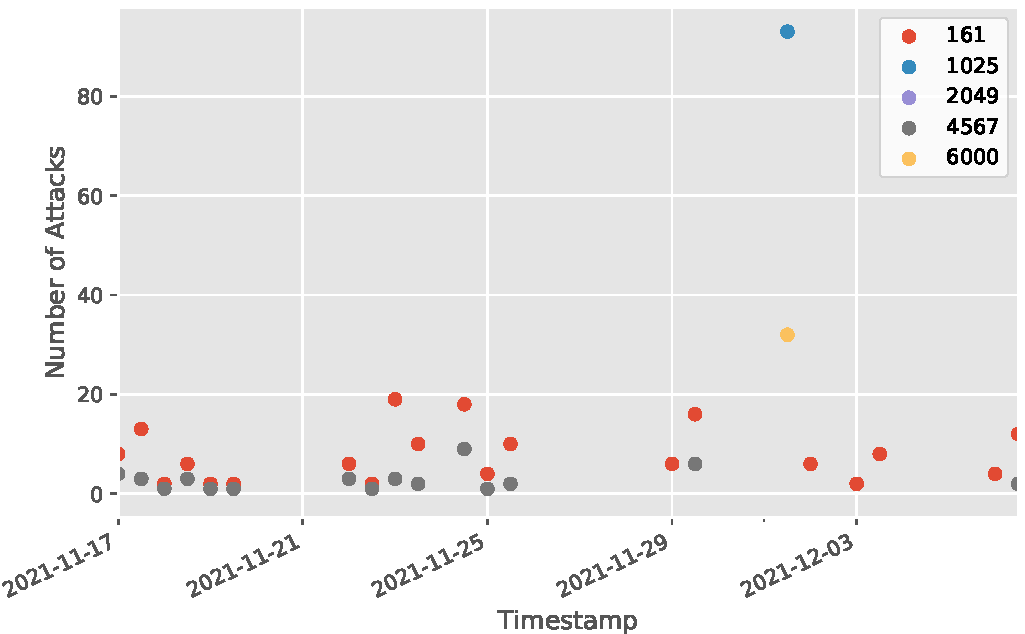
\includegraphics[width=\textwidth]{figures/madcat-port-histogram.pdf}
    \caption[Attack port histogram of T-Pot]{
        Attack port histogram of T-Pot.
        Timestamp; from 16th of November to 7th of December.
    }
    \label{fig:port-histogram}
\end{figure}

% ====================================================================================================================
% T-Pot
Results from the T-Pot instance are exiguous, and in short, no real attacks such as shell exploitation have been performed.
All connection attempts originated from Germany within the same network and are made on ports $161$ and $4567$.
Conpot registered minor SNMPv2 Get, SNMPv1 Get, and GetNext requests.
A possible attack vector could be an \ac{snmp} reflection/amplification attack.
As previously discussed, the assumption is that devices within the network have a misconfigured printer and send broadcast requests frequently to find the machines.
This \ac{snmp} requests affiliate with day-to-day traffic in an internal network, and thus, are not suspicious.
The second most attacked honeypot is Honeytrap which received numerous packets on different ports, whereas $39\%$ evince an empty payload.
All of these received packets have a resolved IP address in the subnet \ipAddress{129.206.0.0/16}.
It remains unclear if these connections are malicious or are acquired by accident.
Investigating the payload of outliers does not confirm the assumption of a vicious intention.
Thus, declaring these results as negligible.
Overall, most of the connection attempt received by the instance are from these IP addresses: \ipAddress{129.206.217.118}, \ipAddress{129.206.218.23}, and \ipAddress{129.206.218.194}.

\begin{figure}
    \lstinputlisting[language=bash, caption={[MADCAT connection attempt to exploit SMB connection]MADCAT connection attempt to exploit SMB connection. Received on the 16th of November. IP reputation: known attacker. Location Germany.}, label={lst:smb-exploitation}]{listings/exploit-smb.txt}
\end{figure}

Lastly, the results from the eduroam network are considered.
Neither T-Pot nor MADCAT could identify any significant behavior for three weeks.
Unlike the subnet \ipAddress{129.206.218.0/24}, the honeypot did not register any suspicious packets, TCP flags, or other \acp{cve}.
In retrospect, the eduroam configuration has been shown to work as designed.
Thus, the client seemed to be encapsulated from others and received no other packets.

Besides the subtle output it has received, the results have given an insight into the value of honeypots in a restricted network zone.
For Heidelberg University, using honeypots to evaluate their stateless firewall has never been considered.
The initial concept has shown that it delivered minor findings in the subnet \ipAddress{129.206.218.0/24} with stage 1 firewall.
As a result, the port 113 used for the IDENT protocol will be removed in the future to reduce the attack surface, thus, contributing to the firewall definition.
Overall, the two instances received numerous packets containing interesting payloads.
Compared to the T-Pot, which has been used in heiCLOUD, results are as expected delicate, and data analysis turns out to be more detailed.
The statement from \citet{Spitzner2003} that honeypots only receive little input and nearly every input is suspicious matches the results only halfway.
As shown beforehand, the results are dramatically little; however, only a few requests seemed suspicious.
Nonetheless, the initial question of whether attackers have access to the restricted network zone at the Heidelberg University has been answered.

\section{Discussion}

This chapter has shown that honeypots help find potential leaks in restricted network zones.
Though, it remains questionable if the concept can deliver accurate results.
The instance has been running for three weeks in the two different subnets.
The honeypot has to be detected as a vulnerable target to deliver meaningful data.
However, it could not detect any large scans on the instance; thus, it is very likely that either an attacker could not find the instance or no one had any access.
In the eduroam network, large scans are negligible due to the firewall permits.
It can be assumed that the results are accurate and do not show any discrepancy.
Considering the subnet with stage one institute firewall, it identified attacks on port 113, resulting in an adaption of the stage one permits.
On the contrary, it could not register any other odd packets on other ports.
A detailed investigation could resolve whether the honeypot is available to attackers.
A misconfiguration of the university firewall has been detected which proves this assumption.

In December, from the 21st to the 23rd, a misconfiguration of the university firewall resulted in a flood of attacks.
In total, the T-Pot instance received \numprint{46328} attacks in three days.
It turns out that five ports were open during that time, allowing attackers to probe the instance (\autoref{fig:tpot-misconfig-port-histogram}).
The most attacked honeypots are RDPY ($58.58\%$), Honeytrap ($24.53\%$), and Cowrie ($11.69\%$).

\begin{figure}
    \centering
    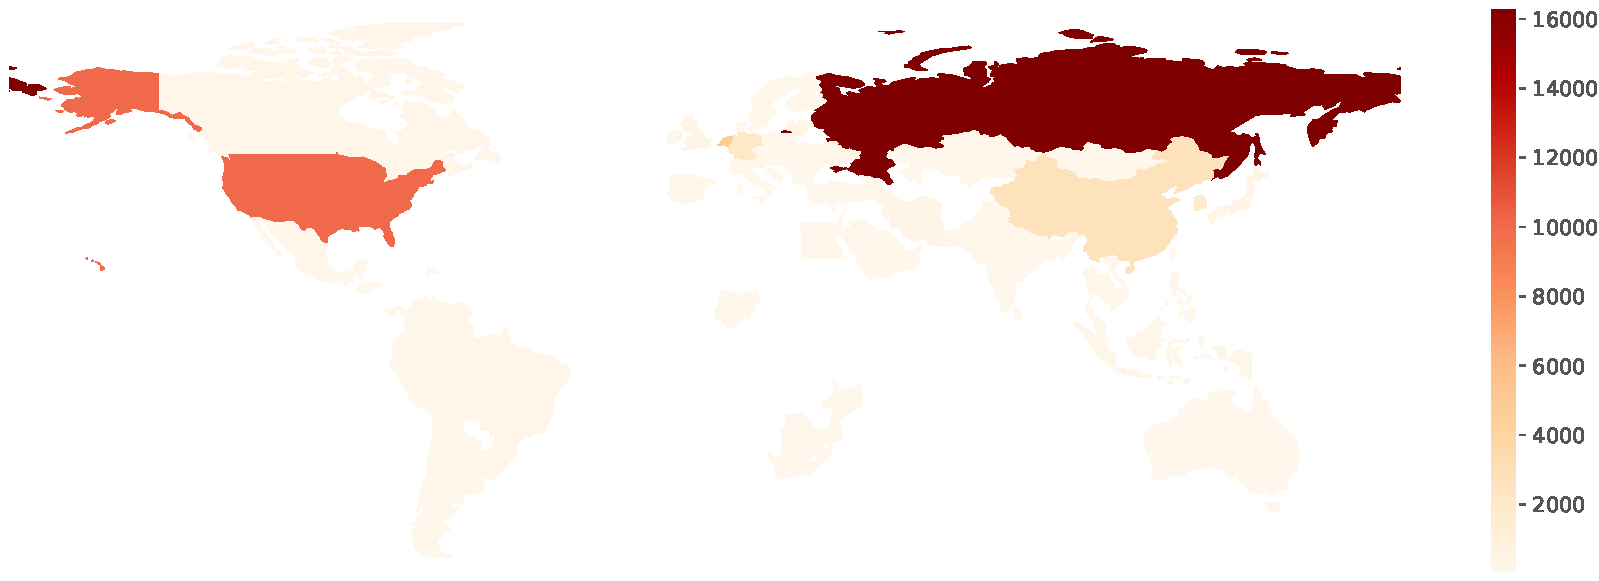
\includegraphics[width=\textwidth]{figures/tpot-misconfig-overview-map.pdf}
    \caption[Attack distribution of MADCAT]{
        Attack distribution of MADCAT.
        USA, Russia, China, and Germany are the most attacking countries.
        Timestamp; from 21st of December to 23rd of December.
    }
    \label{fig:tpot-misconfig-map}
\end{figure}

Like the geographical information of other honeypots, most of the connections originate from the United States, Russia, and China (\autoref{fig:tpot-misconfig-map}).
These similarities indicate a bias of the origin even though the location information is not reliable.

\begin{figure}
    \centering
    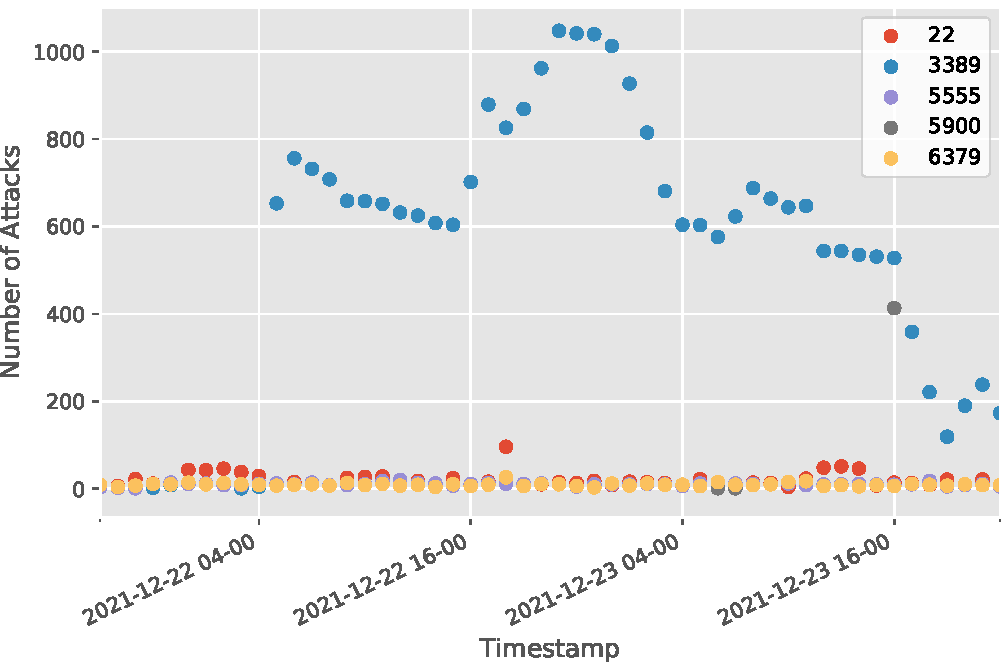
\includegraphics[width=\textwidth]{figures/tpot-misconfig-port.pdf}
    \caption[Attack port histogram of T-Pot]{
        Attack port histogram of T-Pot.
        Timestamp; from 21st of December to 23rd of December.
    }
    \label{fig:tpot-misconfig-port-histogram}
\end{figure}

On RDPY and Honeytrap, many connection attempts on various ports have been made.
Based on the Suricata results, adversaries tried to gain administrator privileges.
For Cowrie, attackers tried to log in and execute commands by brute force or guesswork.
Moreover, the latest crypto-mining malware has been used, which resembles the findings of other honeypots.
These results overlap strongly with those obtained by the T-Pot instance in heiCLOUD.

The firewall administrator stated that the misconfiguration was fixed on the 23rd of December, resulting in a decrease in attacks on the T-Pot instance.
These results have successfully answered our discussion of whether an attacker could detect the host machines at the university building.
It clearly shows that attackers scan these IP address ranges and send malicious packets whenever they can.

